\chapter{Circular Motion in Action}

Swing a bucket of water over your head fast enough, and not a drop spills. Ride a roller coaster through a loop,
and you press into your seat at the bottom and feel nearly weightless at the top. In the Uniform Circular Motion
and Centripetal Force chapter, you learned that anything moving in a circle needs a net force pointing toward the
center. In this chapter, you will use that idea to model real situations: a pig on a string, and a coaster car
whose speed changes as it goes around a loop.

\section{Modeling Circular Motion}
What causes circular motion is a constant force perpendicular to the motion. Consider a satellite circling the Earth. The only force acting on the satellite is gravity, yet the satellite does not fall to the Earth. Why? Let us look at the relative direction of motion and gravity for some different positions of the satellite (we will assume this satellite is moving clockwise from our point of view):
\begin{center}
  \begin{tikzpicture}[scale=0.85, every node/.style={transform shape}]
    \pgfmathsetmacro{\R}{2}
    \pgfmathsetmacro{\Rsat}{3.7}
    \pgfmathsetmacro{\gravlen}{1.4}
    \pgfmathsetmacro{\vellen}{1.5}

    % Earth
    \begin{scope}
      \clip (0,0) circle (\R);
      \shade[ball color=blue!70!cyan] (0,0) circle (\R);
      \fill[sgreen] plot [smooth cycle] coordinates {(-0.3,1.6) (0.7,1.3) (1.1,0.5) (0.5,-0.3) (-0.5,-0.3) (-1.1,0.3)};
      \fill[sgreen] plot [smooth cycle] coordinates {(-1.7,-0.9) (-0.9,-1.1) (-0.5,-1.7) (-1.3,-2.0) (-2.0,-1.5)};
      \fill[sgreen] plot [smooth cycle] coordinates {(1.2,-0.9) (1.8,-0.7) (1.9,-1.4) (1.3,-1.6)};
    \end{scope}
    \draw (0,0) circle (\R);

    % Satellites at N, E, S, W -- orbiting clockwise
    \foreach \a in {90,0,270,180} {
        \pgfmathsetmacro{\sx}{\Rsat*cos(\a)}
        \pgfmathsetmacro{\sy}{\Rsat*sin(\a)}
        \pgfmathsetmacro{\velang}{\a-90}
        \pgfmathsetmacro{\gx}{\sx-\gravlen*cos(\a)}
        \pgfmathsetmacro{\gy}{\sy-\gravlen*sin(\a)}
        \pgfmathsetmacro{\vx}{\sx+\vellen*cos(\velang)}
        \pgfmathsetmacro{\vy}{\sy+\vellen*sin(\velang)}

        % gravitational force arrow (radially inward)
        \draw[->,thick,sred] (\sx,\sy) -- (\gx,\gy);
        % velocity arrow (tangential, clockwise)
        \draw[->,thick,sdkblue] (\sx,\sy) -- (\vx,\vy);

        % satellite icon
        \begin{scope}[shift={(\sx,\sy)},rotate=\velang]
          \draw[fill=sdkblue!60,draw=black] (-0.85,-0.22) rectangle (-0.18,0.22);
          \foreach \gxo in {-0.7,-0.55,-0.4,-0.25} {\draw (\gxo,-0.22) -- (\gxo,0.22);}
          \draw[fill=sdkblue!60,draw=black] (0.18,-0.22) rectangle (0.85,0.22);
          \foreach \gxo in {0.25,0.4,0.55,0.7} {\draw (\gxo,-0.22) -- (\gxo,0.22);}
          \draw[fill=gray!50,draw=black] (-0.18,-0.18) rectangle (0.18,0.18);
        \end{scope}
      }

    % Legend
    \node[sdkblue,anchor=west,font=\bfseries] at (4.4,3.6) {velocity};
    \node[sred,anchor=west,font=\bfseries] at (4.4,3.0) {gravitational force};
  \end{tikzpicture}
\end{center}

No matter what position the satellite is in, the velocity and gravity vectors are perpendicular.

%fix me: section discussing work and delta KE, perpendicular, dot product, no change in v

\begin{Exercise}[title={Circular Motion}, label=circular]
  Just as your car rolls onto a circular track with a radius of 200 m,
  you realize your 0.4 kg cup of coffee is on the slippery dashboard of your
  car. While driving 120 km/hour, you hold the cup to keep it from sliding.

  What is the maximum amount of force you would need to use? (The friction of
  the dashboard helps you, but the max is when the friction is zero.)

\end{Exercise}
\begin{Answer}[ref=circular]
  $$\frac{120 \text{ km}}{1 hour} = \frac{1000 \text{ m}}{1 \text{ km}}\frac{120 \text{ km}}{1 hour} \frac{1 \text{ hour}}{3600 \text{ seconds}}= 33.3 \text{ m/s}$$

  $$F = \frac{m v^2}{r} = \frac {0.4 (33.3)^2}{200} = 2.2 \text{ newtons}$$
\end{Answer}

\begin{Exercise}[title = {Twirling a Whistle}, label = whistle]
  The lifeguard at a local pool is twirling their whistle horizontally. You wonder if the lifeguard could spin the whistle fast enough to break the string. The string the whistle is attached to can hold a maximum mass of 20 kg before breaking. If the lifeguard's whistle string is 0.35 m long and the average whistle has a mass of 165 grams, what is the maximum tangential speed the lifeguard can spin the whistle? How many rotations per second would the whistle be spinning at? Based on this, do you think the lifeguard is capable of spinning the whistle fast enough to break the string?
\end{Exercise}

\begin{Answer}[ref = whistle]
  Givens:
  $$T_{max} = \left( 20 kg \right) \cdot \left( 9.8 \frac{m}{s^2} \right) = 196 N$$
  $$r = 0.35 m$$
  $$m_{whistle} = 165 g = 0.165 kg$$

  Unknown:
  $$v = ?$$
  $$f = ?$$

  Equation(s):
  $$F = ma$$
  $$a = \frac{v^2}{r}$$
  $$v = 2\pi r f$$

  Solution:
  First, we find the tangential speed if the tension in the string is the maximum tension:
  $$T_{max} = m_{whistle}a = m_{whistle} \frac{v^2}{r}$$
  $$v = \sqrt{\frac{T_{max}r}{m_{whistle}}}$$
  $$v = \sqrt{\frac{196 \text{ N} \cdot 0.35 \text{ m}}{0.165 \text{ kg}}} \approx 20.4 \frac{\text{m}}{\text{s}}$$
Therefore, the maximum tangential speed of the whistle before the string breaks is about $20.4$ m/s. The frequency is the number of revolutions per second, which is the speed divided by the circumference $2\pi r$:
$$f = \frac{v}{2\pi r} = \frac{20.4 \text{ m/s}}{2\pi(0.35 \text{ m})} \approx 9.3 \text{ Hz}$$
So the lifeguard would have to swing the whistle at about 9 revolutions
per second to break the string. That is very hard to do by hand, so the
string is probably safe.
\end{Answer}

\begin{Exercise}[title = {The Gravitron}, label = gravitron]
  The Gravitron is a carnival ride where riders "stick" to the wall of a spinning cylinder as the floor beneath them drops away. A video explanation is given here: \url{https://www.youtube.com/watch?v=ifAY5tbYDmQ}. Draw a free body diagram of a rider. If the coefficient of friction between a rider and the wall is 0.32 and the ride is 10 meters across, what angular velocity must the ride reach before the floor drops away?
\end{Exercise}

\begin{Answer}[ref = gravitron]
  There are three forces acting on the rider: gravity, friction with the wall, and the normal force with the wall:

  \begin{center}
    \begin{tikzpicture}
      \draw[thick] (-1, -1) rectangle (1,1);
      \draw[fill=black] (0,0) circle (0.5mm);
      \draw[-latex] (0,0) -- (0, 2) node[above] {$F_f$};
      \draw[-latex] (0,0) -- (3, 0) node[right] {$F_N$};
      \draw[-latex] (0,0) -- (0, -2) node[below] {$F_g$};
    \end{tikzpicture}
  \end{center}

  The FBD lets us write equations for Newton's Second Law in each dimension:
  $$\left( 1 \right) \text{ }ma_x = F_N$$
  $$\left( 2 \right) \text{ }ma_y = F_f - F_g = \mu F_N - mg$$

  Because the rider does not fall down, we know that $a_y = 0 \frac{m}{s^2}$ and therefore equation (2) becomes:
  $$\mu F_N - mg = 0 \to F_N = \frac{mg}{\mu}$$

  Having solved for $F_N$, we substitute for it into equation (1):
  $$ma_x = \frac{mg}{\mu} \to a_x = \frac{g}{\mu}$$

  Since we know $g$ and $\mu$, we can calculate $a_x$:
  $$a_x = \frac{9.8 \frac{m}{s^2}}{0.32} = 30.625 \frac{m}{s^2}$$

  This is the minimum acceleration needed to keep the rider from slipping down. We can now use the relationship between centripetal acceleration, tangential velocity, and the radius to find the angular velocity:
  $$a = \frac{v^2}{r} = \frac{\left( \omega r \right)^2}{r} = \omega^2 r$$
  The ride is 10 meters across, so its radius is 5 meters:
  $$\omega = \sqrt{\frac{a}{r}} = \sqrt{\frac{30.625 \frac{m}{s^2}}{5 \text{ } m}} \approx 2.47 \frac{rad}{s}$$
  That is about 0.4 rotations per second, one turn every 2.5 seconds.
\end{Answer}

\section{Flying Pigs and Tension}
Take a look at the following two videos that involve flying pigs!
\begin{enumerate}
  \item \href{https://youtu.be/vsSID5irx4o}{Flying Pig: Uniform Circular Motion and Centripetal Force}
  \item \href{https://www.youtube.com/watch?v=7WO2DZOsYY4}{flying pig - circular motion [workthrough demo]}
\end{enumerate}

This involves a combination of circular motion and tension. Say the string makes an angle $\theta$ with the vertical and the string of length $L$, causing the pig to move in a circular path with radius $r$. We can draw the following two diagrams for our pig, as shown in Figure~\ref{fig:flyingpig1}.

\begin{figure}[H]
  \centering
  \begin{center}
    \begin{tikzpicture}[>=Stealth,thick,scale=1]
      \node[font=\large] at (0,4.2) {Circular Motion at an angle};

      \draw[dashed, line width=0.8pt] (0,-2.3) -- (0,3.6);

      % gravity arrow
      \draw[->] (2,2.2) -- (2,0.8) node[midway,right] {$g$};

      \draw[dashed] (0,-1) ellipse (3 and 1);

      \draw[->] (0,-1) ++(180:3 and 1)
      arc[start angle=180,end angle=150,x radius=3,y radius=1];
      \draw[->] (0,-1) ++(0:3 and 1)
      arc[start angle=0,end angle=-30,x radius=3,y radius=1];

      \coordinate (P) at (0,3.4);
      \path (0,-1) ++(200:3 and 1) coordinate (M) node[left]{pig};
      \draw (P) -- (M);
      \fill (M) circle (0.12);
    \end{tikzpicture}
  \end{center}
  \caption{The uniform motion of a flying pig attached to a string.}
  \label{fig:flyingpig1}
\end{figure}

% https://www.physicsclassroom.com/class/waves/lesson-0/pendulum-motion
If this is confusing, think of a tetherball from your local playground. It follows the same mechanics!

At any point, we can draw a free body diagram for the pig. Figure~\ref{fig:flyingpig2} shows the forces acting on the pig at all points.
\begin{figure}[H]
  \centering
  \begin{tikzpicture}
    \filldraw (0,0) circle (0.12);
    \begin{scope}[rotate around={-30:(0,0)}]
      \draw[->] (0,0) -- (0,2) node[midway,right] {$F_T$};
      % \draw[->] (0,0) -- (0,-1.5) node[midway,right] {$mg$};
    \end{scope}

    \draw[->] (0,0) -- (0,-2) node[midway,left] {$F_g$};
  \end{tikzpicture}
  \caption{The FBD of the flying pig at any point.}
  \label{fig:flyingpig2}
\end{figure}

To analyze the net forces, the tension force needs to be split into its $x$ and $y$ components. The $y$ component of the tension force must balance out the weight of the pig (as it is not moving vertically), while the $x$ component of the tension force provides the centripetal force to keep the pig moving in a circle.

\[
  \sum F_y = 0 \to F_{T_y} - F_g = 0 \to F_{T_y} = F_g = F_T \cos{\theta} = mg
\]

The centripetal force is found by:
\[
  F_{T_x} = F_c = F_T \sin{\theta} = ma_r = \frac{mv^2}{r}
\]

Dividing the second equation by the first equation gives:
\[
  \frac{F_T \sin(\theta)}{F_T \cos(\theta)} = \frac{\frac{mv^2}{r}}{mg} \to \tan(\theta) = \frac{v^2}{rg}
\]

Solving for $\theta$ gives us $\theta = \arctan\left(\frac{v^2}{rg}\right)$. We can also solve for $v$:
$$v = \sqrt{r g \tan\theta} = \sqrt{L g \sin\theta \tan\theta}$$

Since $r$ can be solved for $\theta$ using $r = L \sin\theta$.

Explicitly, we can express our tension force as $F_T = \frac{mg}{\cos(\theta)}$ (coming from our net force in the $y$-direction).

We can also explicitly solve for $\omega$:
\begin{align*}
  \tan(\theta) & = \frac{v^2}{rg}                               \\
               & = \frac{(r\omega)^2}{rg} = \frac{r\omega^2}{g} \\
  \omega^2     & =\frac{g\tan(\theta)}{r}                       \\
  \omega       & =\sqrt{\frac{g\tan(\theta)}{r}}                \\
\end{align*}

What does all of this tell us?
\begin{itemize}
  \item The vertical component of tension balances the weight of the pig, so there is no vertical motion.
  \item The horizontal component of tension provides the centripetal force that keeps the pig moving in a circle.
  \item The faster the pig moves, the larger the angle $\theta$ and the greater the tension in the string.
  \item The tension is always greater than the pig's weight: $F_T = \frac{mg}{\cos\theta}$.
  \item The angular speed required for a given angle is $\omega = \sqrt{\frac{g\tan\theta}{r}}$. This increases with larger angles, and increases as the radius gets smaller.
\end{itemize}

\begin{Exercise}[label={ex:tetherball}, title={Playground Tetherball}]

  A tetherball of mass .5kg is attached to a string of length 2.5m. When the ball is swung around in a horizontal circle, the string makes an angle of $38^\circ$ with the vertical. If the ball is in uniform circular motion, what is the speed of the ball?
\end{Exercise}
\begin{Answer}[ref={ex:tetherball}]
  Givens:
  \begin{itemize}
    \item Mass of tetherball: $m = 0.5 \text{ kg}$
    \item Length of string: $L = 2.5 \text{ m}$
    \item Angle with vertical: $\theta = 38^\circ$
  \end{itemize}

  The components of the tension force are separated as follows:
  \[
    T\cos\theta = mg,\qquad T\sin\theta = \frac{mv^2}{r}
  \]
  Dividing the second equation by the first equation gives:
  \[
    \tan\theta = \frac{v^2}{rg} \to v = \sqrt{rg\tan\theta}
  \]
  But we are not given $r$. We can find $r$ using trigonometry:
  \[
    r = L\sin\theta
  \]
  Now we can find $v$:
  \[
    v = \sqrt{(L\sin\theta)g\tan\theta}
  \]
  Solving this gives us:
  \[
    v = \sqrt{(2.5\text{ m}\sin 38^\circ)(9.8 \frac{\text{m}}{\text{s}^2})\tan 38^\circ} \approx 3.4 \frac{\text{m}}{\text{s}}
  \]
  The speed of the tetherball is approximately $3.4 \frac{\text{m}}{\text{s}}$.
\end{Answer}

\section{Non-uniform circular motion}
We have talked enough about uniform circular motion, where the speed is constant. However, in many real-world scenarios, the speed is not constant. This is known as \newterm{non-uniform circular motion}. In this case, there are two components of acceleration: the centripetal acceleration $a_\perp$ (toward the center of the circle) and the tangential acceleration $a_\parallel$ (along the direction of motion). The tangential acceleration is responsible for changes in speed, while the centripetal acceleration is responsible for changes in direction. (A swinging pendulum is a good example: it moves along an arc of a
circle, speeding up and slowing down. You will study it in the pendulums
chapter.)

Let us look at a few examples of these concepts in action.
\subsection{Roller Coaster Loop}\index{roller coaster loop}
Now we can talk about a roller coaster. A roller coaster loop is a great example of circular motion. As the roller coaster cart goes through the loop, it experiences both centripetal and tangential acceleration.

We will analyze the cart on a roller coaster at positions at the top, bottom, and sides of the loop, as shown in Figure~\ref{fig:roller_allfour}

\begin{figure}[H]
  \centering
  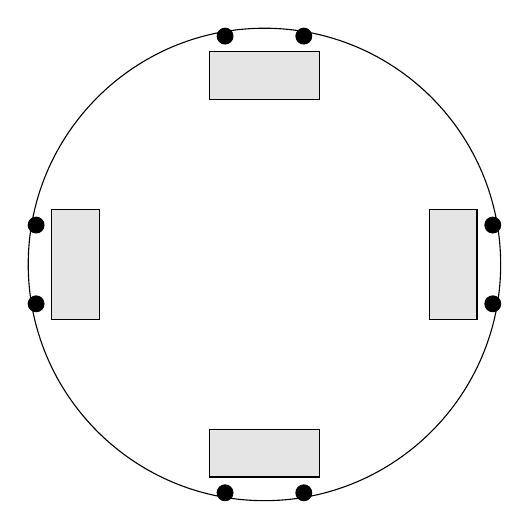
\begin{tikzpicture}
    % ---- Parameters ----
    \def\R{3}           % circle radius
    \def\bw{1.4}        % cart body width
    \def\bh{0.6}        % cart body height
    \def\wr{0.1}        % wheel radius
    \def\wheelDrop{0.2} % distance of wheel below body
    \def\wheelSep{1.0}  % wheel horizontal spacing

    % --- Geometry: where is the wheel center in the cart frame? ---
    % (negative, since wheels are below cart center)
    \pgfmathsetmacro{\wheelCenterY}{-\bh/2 - \wheelDrop}

    % Radial distance of cart center from origin so that the WHEEL
    % lies on the track of radius \R (inside contact):
    % |wheel center| = R - wr
    % => cartR = R - wr + wheelCenterY  (wheelCenterY < 0)
    \pgfmathsetmacro{\cartR}{\R - \wr + \wheelCenterY}

    % ---- Track ----
    \draw (0,0) circle (\R);

    % --- Reusable cart pic (unrotated: wheels downward in -y) ---
    \tikzset{
      cart/.pic={
          % Body
          \draw[fill=gray!20] (-\bw/2,-\bh/2) rectangle (\bw/2,\bh/2);
          % Wheels
          \filldraw (-\wheelSep/2, -\bh/2 - \wheelDrop) circle (\wr);
          \filldraw ( \wheelSep/2, -\bh/2 - \wheelDrop) circle (\wr);
        }
    }

    % ---- Carts on four sides, rotated, with wheels on track ----

    % Bottom (same as your original: cart center at y = -2.4)
    \pic at (0,-\cartR) {cart};

    % Top
    \pic[rotate=180] at (0,\cartR) {cart};

    % Right
    \pic[rotate=90] at (\cartR,0) {cart};

    % Left
    \pic[rotate=-90] at (-\cartR,0) {cart};

  \end{tikzpicture}
  \caption{Carts at four positions around the loop with wheels on the track.}
  \label{fig:roller_allfour}

\end{figure}

\subsection{At the bottom}
At the very bottom of the loop, the forces acting on the cart are gravity and the normal force from the track. Let us imagine the cart goes around the circular track infinitely without ``exiting'' the loop. There must, then, be a force keeping the cart moving in a circle. This force is the centripetal force, which points toward the center of the loop. The only two forces acting on the cart are gravity (downward) and the normal force from the track (upward). We know that a centripetal force must satisfy the formula $F_{net} = F_N - F_g = \frac{mv^2}{r}$. Therefore, the normal force must be greater than the weight of the cart at the bottom of the loop: $F_N = \frac{mv^2}{r} + mg$. This is represented in Figure~\ref{fig:roller_bottom}.

\begin{figure}[H]
  \centering
  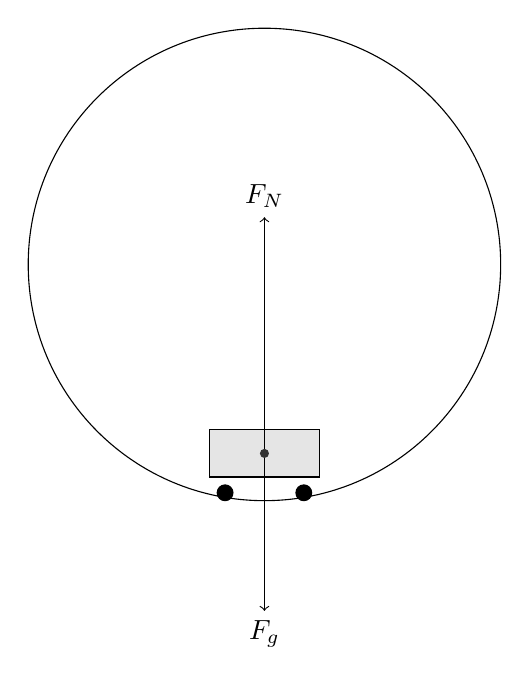
\begin{tikzpicture}
    \def\R{3}           % circle radius
    \def\cartY{-2.4}    % cart vertical position
    \def\bw{1.4}        % cart body width
    \def\bh{0.6}        % cart body height
    \def\wr{0.1}        % wheel radius
    \def\wheelDrop{0.2} % distance of wheel below body
    \def\wheelSep{1.0}  % wheel horizontal spacing
    % Circle centered at (0,0)
    \draw (0,0) circle (\R);
    % Cart position (you only need to change this coordinate)
    \coordinate (car) at (0,\cartY);
    % Draw cart body and wheels relative to (car)
    \begin{scope}[shift={(car)}]
      % Body
      \draw[fill=gray!20] (-\bw/2,-\bh/2) rectangle (\bw/2,\bh/2);
      % Wheels
      \filldraw (-\wheelSep/2, -\bh/2 - \wheelDrop) circle (\wr);
      \filldraw ( \wheelSep/2, -\bh/2 - \wheelDrop) circle (\wr);
    \end{scope}

    \draw[->] (0,\cartY) -- (0, \cartY + 3) node[above] {$F_N$};
    \draw[->] (0,\cartY) -- (0, \cartY - 2) node[below] {$F_g$};

    \filldraw[black!80] (car) circle (0.05);

  \end{tikzpicture}
  \caption{The FBD of the roller coaster at the bottom.}
  \label{fig:roller_bottom}
\end{figure}
\subsection{At the top}
At the very top of the loop, the forces acting on the cart are gravity and the normal force from the track. Both forces point \emph{downward} this time, toward the center of the loop. We can say that $F_{net} = F_N + F_g = \frac{mv^2}{r}$. Solving for the normal force gives: $F_N = \frac{mv^2}{r} - mg$.

Notice that the normal force at the top is smaller than at the bottom.
The normal force can never be negative (the track can push, but not pull),
so $\frac{mv^2}{r} \ge mg$, which means $v \ge \sqrt{rg}$. This is represented in Figure~\ref{fig:roller_top}.

\begin{figure}[H]
  \centering
  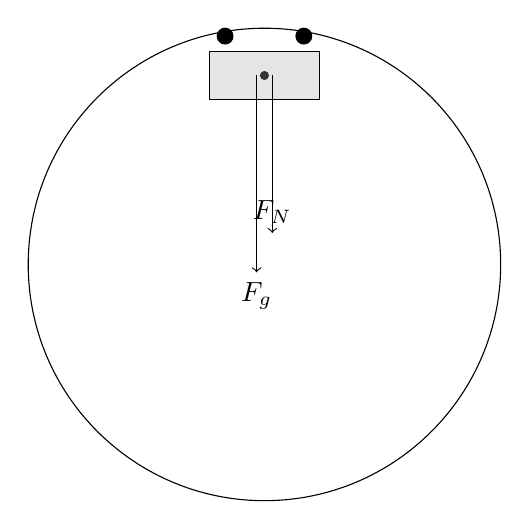
\begin{tikzpicture}
    \def\R{3}           % circle radius
    \def\cartY{2.4}    % cart vertical position
    \def\bw{1.4}        % cart body width
    \def\bh{0.6}        % cart body height
    \def\wr{0.1}        % wheel radius
    \def\wheelDrop{0.2} % distance of wheel below body
    \def\wheelSep{1.0}  % wheel horizontal spacing
    % Circle centered at (0,0)
    \draw (0,0) circle (\R);
    % Cart position (you only need to change this coordinate)
    \coordinate (car) at (0,\cartY);
    % Draw cart body and wheels relative to (car)
    \begin{scope}[rotate around={180:(car)},shift={(car)}]
      % Body
      \draw[fill=gray!20] (-\bw/2,-\bh/2) rectangle (\bw/2,\bh/2);
      % Wheels
      \filldraw (-\wheelSep/2, -\bh/2 - \wheelDrop) circle (\wr);
      \filldraw ( \wheelSep/2, -\bh/2 - \wheelDrop) circle (\wr);
    \end{scope}

    \draw[->] (0.1,\cartY) -- (0.1, \cartY - 2) node[above] {$F_N$};
    \draw[->] (-0.1,\cartY) -- (-0.1, \cartY - 2.5) node[below] {$F_g$};

    \filldraw[black!80] (car) circle (0.05);

  \end{tikzpicture}
  \caption{The FBD of the roller coaster at the top.}
  \label{fig:roller_top}
\end{figure}

So at the top of the loop, the minimum speed to stay on the track is
$v = \sqrt{rg}$. (At the bottom there is no minimum: the track pushes up
harder the faster you go.) If the cart is slower than $\sqrt{rg}$ at the
top, it will lose contact with the track, as there will not be enough normal force to provide the centripetal force needed to keep the cart moving in a circle. Think about where this observation comes from!

\subsection{At the sides}
Now at the sides of the loop (say $0$ and $\pi$ if we view the roller coaster as a unit circle), the net force is directed at an angle. The normal force from the track acts horizontally, pointing toward the center of the circle, while the gravitational force acts vertically downward. Since these two forces are perpendicular to each other, the net force is the vector sum of the normal and gravitational forces.

At the right side ($\theta = 0$), the normal force points leftward (toward the center), and gravity points downward, so the net force points diagonally down and to the left, toward the lower-left quadrant of the circle.

At the left side ($\theta = \pi$), the normal force points rightward (toward the center), and gravity still points downward, so the net force points diagonally down and to the right, toward the lower-right quadrant of the circle.

The normal force provides the centripetal part of the net force, and
gravity provides a tangential part, along the track. Because the net force
does not point straight at the center, the cart's speed changes: on the
side where it is climbing, gravity slows it down; on the side where it is
falling, gravity speeds it up. This is modeled in Figure~\ref{fig:roller_sides}.

\begin{figure}[H]
  \centering
  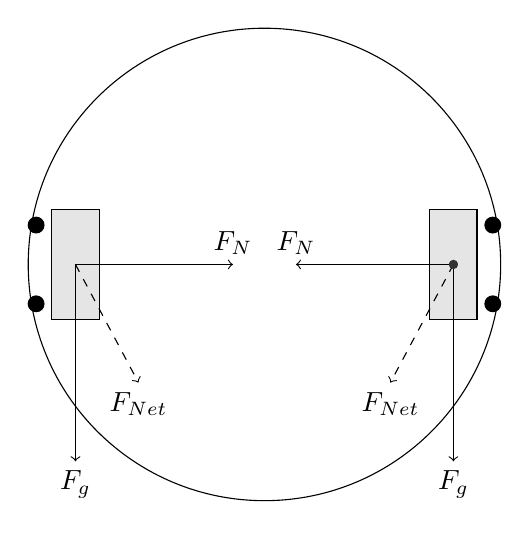
\begin{tikzpicture}
    \def\R{3}           % circle radius
    \def\cartY{0}    % cart vertical position
    \def\bw{1.4}        % cart body width
    \def\bh{0.6}        % cart body height
    \def\wr{0.1}        % wheel radius
    \def\wheelDrop{0.2} % distance of wheel below body
    \def\wheelSep{1.0}  % wheel horizontal spacing
    % Circle centered at (0,0)
    \draw (0,0) circle (\R);
    % Cart position (you only need to change this coordinate)
    \coordinate (car) at (2.4,\cartY);
    % Draw cart body and wheels relative to (car)
    \begin{scope}[rotate around={90:(car)},shift={(car)}]
      % Body
      \draw[fill=gray!20] (-\bw/2,-\bh/2) rectangle (\bw/2,\bh/2);
      % Wheels
      \filldraw (-\wheelSep/2, -\bh/2 - \wheelDrop) circle (\wr);
      \filldraw ( \wheelSep/2, -\bh/2 - \wheelDrop) circle (\wr);
    \end{scope}

    \draw[->] (2.4,\cartY) -- (.4, \cartY) node[above] {$F_N$};
    \draw[->] (2.4,\cartY) -- (2.4, \cartY - 2.5) node[below] {$F_g$};
    \draw[->, dashed] (2.4,\cartY) -- (1.6, \cartY - 1.5) node[below] {$F_{Net}$};

    \filldraw[black!80] (car) circle (0.05);

    \begin{scope}[rotate around={-90:(-2.4, \cartY)},shift={(-2.4, \cartY)}]
      % Body
      \draw[fill=gray!20] (-\bw/2,-\bh/2) rectangle (\bw/2,\bh/2);
      % Wheels
      \filldraw (-\wheelSep/2, -\bh/2 - \wheelDrop) circle (\wr);
      \filldraw ( \wheelSep/2, -\bh/2 - \wheelDrop) circle (\wr);
    \end{scope}

    \draw[->] (-2.4,\cartY) -- (-.4, \cartY) node[above] {$F_N$};
    \draw[->] (-2.4,\cartY) -- (-2.4, \cartY - 2.5) node[below] {$F_g$};
    \draw[->, dashed] (-2.4,\cartY) -- (-1.6, \cartY - 1.5) node[below] {$F_{Net}$};

    \filldraw[black!80] (car) circle (0.05);

  \end{tikzpicture}
  \caption{The FBD of the roller coaster at the sides.}
  \label{fig:roller_sides}
\end{figure}


\begin{Exercise}[title={Roller Coaster Loop}, label=rollercoaster]
  This question is taken from the AP Physics C Review Book, 19th edition.

  A roller-coaster car enters the circular loop portion of the ride. At the very top of the circle (where people are upside down), the car has a speed of $25$ m/s, and the acceleration points straight down. If the diameter of the loop is $50$ m and the total mass of the car plus passengers is $1,200$ kg, find the magnitude of the normal force exerted by the track on the car at this point. Also find the normal force exerted by the track on the car when it is at the very bottom of the loop, given it is still traveling at $25$ m/s. You may use $g=10$ m/s$^2$ for simpler calculations.
\end{Exercise}

\begin{Answer}[ref=rollercoaster]
  \begin{itemize}
    \item At the top of the loop:
          At the top of the loop, both the gravitational force and the normal force point downward. Therefore, we can write:
          $$F_{net} = F_N + F_g = \frac{mv^2}{r}$$
          Solving for the normal force gives:
          $$F_N = \frac{mv^2}{r} - F_g$$
          Substituting for $F_g = mg$ (using $g = 10$ m/s$^2$ for this problem) and $r = \frac{d}{2} = 25$ m:
          $$F_N = \frac{(1200 \text{ kg})(25 \frac{m}{s})^2}{25 \text{ m}} - (1200 \text{ kg})(10 \frac{m}{s^2})$$
          $$F_N = 30000 \text{ N} - 12000 \text{ N} = 18000 \text{ N}$$

    \item At the bottom of the loop:
          At the bottom of the loop, the gravitational force points downward while the normal force points upward. Therefore, we can write:
          $$F_{net} = F_N - F_g = \frac{mv^2}{r}$$
          Solving for the normal force gives:
          $$F_N = \frac{mv^2}{r} + F_g$$
          Substituting for $F_g = mg$ (using $g = 10$ m/s$^2$ for this problem) and $r = \frac{d}{2} = 25$ m:
          $$F_N = \frac{(1200 \text{ kg})(25 \frac{m}{s})^2}{25 \text{ m}} + (1200 \text{ kg})(10 \frac{m}{s^2})$$
          $$F_N = 30000 \text{ N} + 12000 \text{ N} = 42000 \text{ N}$$
  \end{itemize}
\end{Answer}
Our next chapter will explore oscillations, restoring forces, simple harmonic motion, and more concepts of harmonic motion.
